%!TEX root = ../dissertation.tex
\chapter{Materials \& Methods}
\label{chap:02}

\Lettrine{Computational chemistry} was first coined by Schleyer at a conference in 1966 to refer to Allinger’s work on molecular mechanics, separating it from other studies that would fall under the ‘theoretical chemistry’ category at that time. Nowadays, the term is broader and considers far more techniques. In fact, under the modern definition earlier works would be considered ‘computational chemistry’; albeit analog ones. In 1930, Kettering and more researchers in General Motors, built ball-and-spring models for several molecules and correlated their vibration modes with their Raman spectra. This work, titled ‘A representation of the dynamic properties of molecules by mechanical models’ could be considered one of the first ‘molecular modeling’ works.

\section{Origins of molecular modeling}
% \addcontentsline{toc}{section}{Origins of molecular modeling}
The birth of theoretical chemistry, from a quantum chemistry perspective, can be pinpointed with the description of the Schrödinger equations in 1925-1926 $ \{ $ $ \} $ . The first application of quantum mechanics came a year later, in 1927, with the publication of Burrau’s studies on H2+ $ \{ $ burrau1927$ \} $  and Heitler and London calculations on H2 $ \{ $ Heitler $\&$  London, 1927$ \} $ . The field began to grow rapidly (Teller $ \{ $ $ \} $ , Mulliken $ \{ $ $ \} $ , Born $ \{ $ $ \} $ , Oppenheimer $ \{ $ $ \} $ , Pauling $ \{ $ $ \} $ , Hückel $ \{ $ $ \} $ , Hartree $ \{ $ $ \} $ , Fock $ \{ $ $ \} $ $ \ldots $ ) and computational implementations of the new theoretical framework started to be feasible after the advances in computer technology during the late 40s $ \{ $ $ \} $ . In the 50s and 60s, several milestone papers were published, making for the first documented computational chemistry calculations (refer to $ \{ $ https://onlinelibrary.wiley.com/doi/10.1002/9780470125823.ch1$ \} $  and CCL conversation $ \{ $ http://www.ccl.net/cgi-bin/ccl/message-new?2018+04+19+002$ \} $  for further information). Also, non-quantum, classical approaches stemming from theoretical physics started to emerge, although not strictly dealing with chemistry problems $ \{ $ Alder1959,Gibson1960,Rahman1964$ \} $ .

By the 70s, several journals had appeared to target computational chemistry and the first quantum chemistry packages began to be distributed (including the first version of the now ubiquitous Gaussian $ \{ $ $ \} $ ). The available hardware back then only allowed for ab initio\footnote{ A model is said to be ab initio when it only considers the resolution of the first principle equations (Schrödinger’s), without support from experimental observations. Empirically derived models do take these observations into account, very often as a workaround to avoid solving the full equation system. When the two approaches are combined, those are semi-empirical methods.  } calculations of molecules as big as naphthalene and azulene (18 atoms). In those same years, molecular mechanics methods became more popular, especially with the contributions by Lifson’s CFF $ \{ $ Warshel1969, Hagler et al., 1974; Hagler and Lifson, 1974; Niketic and Rasmussen, 1977$ \} $ , Allinger’s MM series $ \{ $ Allinger1973, Allinger1977$ \} $ , Scheraga’s ECEPP potentials $ \{ $ Momany et al.,1975; Némethy et al., 1983$ \} $ , Karplus’ CHARMM $ \{ $ brooks1983$ \} $ , van Gunsteren’s GROMOS $ \{ $ 1978$ \} $  and others, proving the power of empirical parameterization. By the 80s, Computer Assisted Molecular Design (CAMD) was the new hype that would revolutionize the pharmaceutical industry $ \{ $ Next Industrial Revolution: Designing Drugs by Computer at Merck, Fortune cover 1981$ \} $ , and by the 90s it was clear that computational chemistry was broader than quantum chemistry. In the preface of Reviews in Computational Chemistry Volume I $ \{ $ Kenny B. Lipkowitz, Donald B. Boyd, 1990$ \} $ , editors acknowledge that \textit{$``$[$ \ldots $ ] we do not view the terms theoretical chemistry and computational chemistry as synonymous. Computational chemistry sometimes involves application of computerized algorithms from quantum theory, but computational chemistry is certainly more than quantum chemistry [$ \ldots $ ]. Molecular mechanics, molecular dynamics, computer graphics, molecular modeling, and computer-assisted molecular design are other important aspects of computational chemistry [$ \ldots $ ]$"$ .}

Nowadays, molecular modeling encompasses techniques and strategies beyond what is traditionally considered computational chemistry (this is, quantum and molecular mechanics, mainly). While a brief overview was already given in \autoref{chap:01}, more details are needed to fully comprehend the applicability of each method. However, this chapter is not intended as a manual on any of these methods, but a reasonably complete introduction to the numerous molecular modeling manifestations.

% [FIGURE: Timeline of molecular modelling milestones] TODO!

\section{State of the art of molecular modeling }
% \addcontentsline{toc}{section}{State of the art of molecular modeling }
These light notions on the history of molecular modeling introduced a key concept in model categorization: the \textit{theory level}, an estimation of the complexity of the theory supporting the method, that while arbitrary, gives a quick understanding of the intricacies involved. Higher theory levels usually refer to highly accurate, computationally demanding methods that rely on complex mathematical models. Lower theory levels, on the contrary, refer to less accurate and computationally cheap methods relying on simpler models.

In addition to quantum mechanics and molecular mechanics, after decades of progress, the currently available modelling toolbox is a rather diverse set of software utilities that apply very different theories, simplifications and approaches to deal with very particular problems. There are also a lot of different areas where they can be applied, and depending on the originating field, a very different mindset has permeated into the model. The following pages will introduce the major families of software approaches in computational chemistry and molecular modelling. They will be listed in two major groups depending on the focus (energy description or search space exploration), and in descending order of level of theory, which, in practice, means going from high-accuracy to lower-accuracy methods.

Lists: https://www.click2drug.org/index.html, https://omictools.com/

\subsection{Methods focused on energy description}
% \addcontentsline{toc}{subsection}{Methods focused on energy description}
\subsubsection{Quantum Mechanics (QM)}
% \addcontentsline{toc}{subsubsection}{Quantum Mechanics (QM)}
The main idea behind quantum chemistry is that molecules and, by extension, all ordinary matter, can be viewed as composed only of positively charged nuclei and negatively charged electrons. Mathematically, this can be expressed with the time-independent Schrodinger equation:

 \[ H \Psi =E \Psi =T_{n}+T_{e}+V_{ne}+V_{ee}+V_{nn} \]

, where $H$ is the Hamiltonian operator, $E$ is the total energy of the system, $T_{n}$ and $T_{e}$ are the kinetic energies of nuclei and electrons, respectively, and $V_{ne}$, $V_{ee}$ and $V_{nn}$ are the potential energy between nuclei and electrons, electrons against each other, and nuclei against each other, respectively. Solving this equation for any system would mean seeking the eigenfunctions and eigenvalues of that Hamiltonian.

The details of such resolution are out of the scope of this thesis, but some comments can be made about its practical effects. Since only one-particle and two-particle systems can be solved analytically, numerical methods are employed to approximate the solution for systems of 3 or more particles: the many-body problem. While not analytical, the same methods can be applied iteratively to any given precision; the only restraints are computational and time resources. As a result, some approximations have been developed over the years to simplify the equation solving process without much accuracy loss.

The first approximation to appear was the Born-Oppenheimer approximation. It relies on the big mass difference between nuclei and electrons. In hydrogen, the monoprotonic nucleus is already 1800 times heavier than the electron; for uranium, the nucleus/electron mass ratio goes up to 430,000. This leads to consider that, given the enormous mass difference, electrons and nuclei move in different time-scales: if the nucleus moves, the electrons would follow ‘instantaneously’. This means that the nucleus can be considered stationary for electronic timescales, and appear as parameters in the equation, greatly simplifying its solution.

Even with uncoupled motions, the dynamics of electrons are complex and require advanced computational methods. A significant simplification would be to treat electrons as independent from each other by introducing a ‘independent-particle’ model, either by neglecting all interactions altogether, or, even better, by introducing an average interaction factor: the Hartree-Fock (HF) theory. In HF methods, electronic interactions are not explicitly described, but with a large basis set$\ast$  99$\%$  of the energy can be described by the HF wave function. The difference between the energy predicted by (Restricted) HF calculations and the real energy is called ‘electronic correlation’, which in certain chemical phenomena is key to obtaining accurate predictions. As a result, three main strategies have been developed to calculate it explicitly: Configuration Interaction (CI), Many-Body Perturbation Theory (MBPT) and Coupled Cluster (CC).

Evidently, these methods involve extra computational complexity, so in some cases, more aggressive approximations have been applied. This is the case of semi-empirical methods, which instead of trying to resolve some of the most complex integrals, resort to experimental parametrization of the results. While it is true that this leads to less accurate results, they are way faster and, with sensible parameters, the difference can be neglected depending on the study at hand.

HF theory is not the only applicable approximation to simplify the many-electron problem. In a way, Density Functional Theory (DFT) can be seen as a more efficient strategy to tackle the challenge. DFT is based on the Hohenberg and Kohn proof, which suggests that the ground state electronic energy can be determined completely by the electron density. This is, knowing the electron density leads to knowing the energy unequivocally. The only unknown here is guessing that correspondence, expressed as a functional\footnote{Not to be confused with a function: a function takes variables and produces numbers; a functional takes functions and produces numbers out of them.} or function of function(s). As opposed to HF methods, where the complexity of a wave function increases exponentially with the number of electrons, in Orbital-Free DFT, the electron density has always the same number of variables, independent of system size. However, describing the kinetic energy with a functional of the density is not accurate enough for the current demands of computational chemistry, so the most used approach today, based on the Kohn-Sham Theory, reintroduces orbitals to calculate the kinetic energy. This has three consequences: (1) accuracy is dramatically increased, (2) the complexity grows from 3 variables to 3N, (3) electronic correlation must be calculated separately.

Since HF-style orbitals now give 99$\%$  of the correct kinetic energy, the remaining energy can be absorbed in the correlation term, which is still calculated through an unknown functional. Even with higher complexity (N->3N) than Orbital Free DFT, it still less complex than the HF methods that explicitly consider electronic correlation. Thus, KS-DFT methods are generally preferred: the offer a computational cost similar to HF theory, but with the possibility of providing more accurate results. They need a good exchange-correlation functional, though, which can only be obtained exactly for the free electron gas; for other cases, approximations must be employed, like local-density (LDA), local spin-density (LSDA) or generalized gradient (GGA, meta-GGA) approaches.

All these methods are applied to solve the time-independent Schrodinger equation; this is, to obtain the energy of a system with given coordinates. If the dynamics of the system (i.e. evolution along time) must be studied, the time-dependent equation must be solved, which involves highly complex calculations to obtain reasonable accuracy. With current resources, only di- and triatomic species can be simulated this way. Additional atoms would need to be frozen or treated classically.

A workaround would involve a semi-classical approach. In Ab Initio Molecular Dynamics (AIMD), electrons are treated quantum-mechanically, and nuclei, classically (Born-Oppenheimer Molecular Dynamics, BOMD). At each time step, a converged wave function is obtained and the corresponding nuclear gradients are used to propagate the time-evolution. However, for accurate results, one must resort to tightly converged wave functions (in BOMD) or very small timesteps (in Car-Parrinello Molecular Dynamics, CPMD).

\subsubsection{Force fields: Molecular mechanic, Molecular dynamics and Metadynamics}
% \addcontentsline{toc}{subsubsection}{Force fields: Molecular mechanic, Molecular dynamics and Metadynamics}
Depending on the phenomena under study, explicit consideration of electrons is not always necessary. If that’s the case, the Schrodinger equation can be bypassed and \textbf{the electronic energy can be written as a parametric function of the nuclear coordinates}. Those parameters are fitted to reproduce either experimental measurements or results obtained with higher levels of theory (i.e. QM). The set of parameters needed to write the set of equations is called ‘force field’, and the theory behind this strategy is called ‘Molecular mechanics’ (MM). Given the size of nuclei, these can be treated classically with Newton’s second law with sufficient accuracy, resulting in equations much simpler than their QM counterpart, which allow faster computations and, as a result, dealing with larger systems (tens of thousands of atoms). Neglecting the existence of electrons has some consequences, though: bonding information is lost and must be provided explicitly, rather than being an inherent result of the equation.

In MM, molecules are described by a ‘ball and spring’ model: atoms are abstracted as spheres of given radius and ‘softness’, and bonds have length and ‘stiffness’. In such an ensemble, the potential energy of the system can be described as the sum of several components: stretching, bending, torsions, non-bonding interactions (usually, Van der Waals and Coulomb), and a cross-term of the first three.

 \begin{align}
	E_{FF}=E_{stretching}+E_{bending}+E_{torsional}+E_{non-bonding}+E_{cross} \\ \tag{Force field energy}
\end{align}

If each of the terms can be expressed as a function of the coordinates for the involved atoms, the potential energy can be obtained, and geometries and relative energies can be calculated by optimization. Thus, all that remains is to obtain the parameters for each type of interaction involved in the system under study. Fortunately, most molecules can be described as a composition of a small set of functional subunits or groups, the properties of which rarely change. For example, all C=O bonds are around 1.22A long. Instead of having to parameterize each type of atom and bond for each type of molecule, these similarities allow to construct set of parameters with reasonable easiness, in principle.

As opposed to QM, these equations can be solved efficiently enough to consider time-dependent analysis. If one takes the force field equations and calculates the resulting forces and velocities, the position of the atoms can be figured out with high accuracy if the timestep is small enough (i.e. in the same order of magnitude as the smallest perturbation studied: hydrogen vibration, in the order of femtoseconds). This strategy gives rise to a field called Molecular Dynamics, which allows to study the behavior of molecules along time. Modern computer architectures allow to resolve each timestep around 10\textsuperscript{8 }times daily! Processes involving seconds in real-life can be calculated within a month.

Gaining access to such magnitudes allows to calculate properties not available in other higher levels of theory: conformational changes, binding pathways, or thermodynamic magnitudes such as free energy. However, in those calculations the potential energy surface (PES) must be well-sampled. Several methods account for this issue, such as metadynamics (MTD), umbrella sampling or adaptively-biased MD. In the case of MTD, the system is assumed to be describable by a few collective variables or reaction coordinates, which are then explored in such a way that revisiting sampled states is discouraged.

\subsubsection{QM/MM}
% \addcontentsline{toc}{subsubsection}{QM/MM}
Dealing with big systems (more than 300-500 atoms) with QM techniques is not feasible due to computational restraints. In some cases, though, only a subset of the system actually needs explicit consideration of the electrons. One strategy would consist of pruning the nonimportant parts, replacing them by smaller functional units which would keep the system’s $``$chemical identity$"$ .

In other studies, like enzyme reactivity, the nonreactive part of the enzyme is assumed to be important in keeping the active site conformation, and as such, cannot be pruned out. While some authors do model enzyme reactivity with a prune-and-freeze strategy $ \{ $ Himo$ \} $ ,\ a large part of the research community prefers to consider all the protein in the calculation.  This can be approached with QM/MM methods, in which the reactive atoms and its immediate surroundings are studied with QM, while the rest of the system is treated classically. The energy of the system is then calculated as a sum of the QM energy, the MM energy and the interaction between both.


\begin{align}
	E_{total}=E_{QM}+E_{MM}+E_{QM/MM} \\ \tag{QM/MM energy}
\end{align}


The independent QM and MM terms can be calculate straightforwardly as explained before, but deciding on how to calculate the interaction is not as intuitive. In general, three strategies can be applied: (1) mechanical embedding, which only considers bonded and steric effects; (2) electrostatic embedding, which also considers the electric field of the MM part; and (3) polarizable embedding, which also adds polarizabilities between the QM and MM parts. Even in the simplest case, mechanical embedding, technical difficulties may arise if a bond is cleaved by the QM/MM partitioning, which would require balancing the unpaired electrons in the QM part by adding a hydrogen ‘link’ atom invisible to the MM part. Similarly, the dangling bond in the MM part must be dealt somehow, normally adding the needed stretching, bending and torsional terms.

Mixing methods of different level theories for a single system is generalized in the ONIOM approach, which assumes additivity of the different ‘layers’. For two layers, it classifies the system in ‘model’ (the subset of the system which is dealt with a higher level of theory) and ‘real’ (the full model, including the ‘model’ subset). The ‘model layer’ is calculated both with the higher level of theory (usually QM) and the lower one (usually a force field), while the real layer is only calculated with the lower level of theory. Then, the energy is given as:

\begin{align}
  E_{ONIOM}=E_{high}^{real}=E_{high}^{model}-E_{low}^{model}+E_{low}^{real} \\ \tag{ONIOM energy}
\end{align}


Another intrinsic problem to QM/MM methods is the sampling. As the contribution of the MM part to the QM/MM energy is larger than the QM due to the number of atoms involved (around 100 in QM or 1,000-10,000 in MM), reported energy will be very sensitive to even small changes in the MM layer. As a result, when an energy profile must be calculated, the MM part is kept rigid during the whole process, which requires a carefully chosen initial structure to begin with. This usually involves a protocol where a long MD run is performed to obtain a representative snapshot of the simulation.

% [Figure: ONIOM scheme] % TODO!

\subsection{Methods focused on search space exploration}
% \addcontentsline{toc}{subsection}{Methods focused on search space exploration}
\subsubsection{Spatial exploration: normal modes $\&$  docking (protein-ligand docking)}
% \addcontentsline{toc}{subsubsection}{Spatial exploration: normal modes $\&$  docking (protein-ligand docking)}
Even with latest advances in computer architecture and software improvements to make the most out of it, some potential energy surfaces are too vast and complex to be explored efficiently with molecular dynamics, let alone quantum dynamics. While this might not apply in the next decade, techniques that take educated shortcuts to traverse broad conformational spaces are still necessary. This is particularly true in large molecules such as proteins, where structural fluctuations occur at very different time scales and amplitudes: local motions take place are fast and short (10\textsuperscript{-15} to 10\textsuperscript{-1}s, 0.01-5A), and collective motions are slow and long (10\textsuperscript{-9} to 1s, 1-10 \AA). This category is too broad to be analyzed exhaustively, but two approaches can be highlighted due to their popularity: normal modes analysis (NMA) and docking procedures.

In NMA, slow, collective motions of a molecular structure can be approximated through the composition of its independent (normal) harmonic oscillations (modes). NMA approach is parallel to MM in its theoretical support, meaning that bonds are replaced by ‘springs’ or harmonic oscillators. As a result, the mathematical treatment consists of finding the eigenvalue of each coupled oscillator, which is simple enough to be calculated efficiently for thousands of atoms. In fact, there is no obligation to treat each atom and bond independently, as nearby atoms can be grouped together in a new body to reduce the needed number of oscillators (coarse-grained NMA). All these approximations allow dynamic insights on the movements of a macromolecule without the technical limitations of MD, which require long runs to observe slowest motions. Since NMA does not consider time at all and only requires an initial structure on which to compute the normal modes, the vibrations obtained only apply to that particular conformation. In other words, only the local potential energy wells are explored, which can provide a short-sighted analysis if no other conformations are assessed.

Recognition processes involve large conformational changes and are key in research areas such as drug development or metabolic studies. Again, MD principles should be able to simulate them with long runs, and would definitely be the way forward in the near future $ \{ $ \href{http://onlinelibrary.wiley.com/doi/10.1002/wcms.1320/full}{http://onlinelibrary.wiley.com/doi/10.1002/wcms.1320/full}$ \} $ , but since the 90s a different shortcut was devised. Docking techniques were developed to describe feasible binding modes of small molecules (ligands) within a bigger macromolecule (the host, which is normally a protein). To do that, potential binding pockets in the host are explored explosively by placing the ligand in random orientations and positions (rigid body transformations), contemplating some internal flexibility if necessary (through torsions in the small molecule or rotamer exchange for the side chains in the protein), and finally assessing their non-bonding interactions. Since the spatial landscape needs to be explored efficiently, with thousands of attempts before finding a good pose, the energy representation is often cruder than in higher levels of theory in honor of speed and efficiency: the scoring function. While in principle it could use a full MM force field $ \{ $ $ \} $ , most popular approaches resort to simplifications, like knowledge-based parameters obtained out of structural databases $ \{ $ PDB$ \} $  or empirical evidences $ \{ $ $ \} $ . Other approaches resort to shape complementarity between the Van der Waals surfaces of the involved molecules and, more recently, to Artificial Intelligence (AI) deep learning techniques $ \{ $ $ \} $ .

Docking techniques can also involve other type of molecules, like protein-protein or protein-nucleic acid studies. In this variant, more approximations are needed due to the broader conformational space involved, like only considering rigid-body transformations.

\subsubsection{Chemogenetic exploration (assess mutation stability, chemical functionalization$ \ldots $ )}
% \addcontentsline{toc}{subsubsection}{Chemogenetic exploration (assess mutation stability, chemical functionalization$ \ldots $ )}
Of all the techniques detailed until know, only QM studies allow topology changes like bond breaking or creation. This is, when dealing with MM, NMA or docking, most approaches will assume that the starting set of atoms and their connectivity will be the same during the whole simulation. As a result, to assess different variants of the same compound one must run the same protocol separately for each variant.

The most popular technique employing this strategy is virtual screening, which essentially performs docking calculations for massive datasets of drug-like compounds. In most implementations, the database must be built beforehand and the chemical space is only explored by trying different entries in the dataset. This is, no algorithmic modification of the structure is done during the simulation. With big enough datasets, sampling should not be a problem, but some studies point out that the chemical space explored this way is very limited $ \{ $ mapa de calor usado en el master$ \} $ .



\begin{itemize}
	\item https://www.sciencedirect.com/science/article/pii/S0079610714000960

	\item https://www.nature.com/articles/nrd.2016.213

	\item https://www.thieme-connect.com/products/ejournals/abstract/10.1055/s-0034-1396322

	\item https://pubs.acs.org/doi/abs/10.1021/ar500432k

	\item https://www.nature.com/articles/nmeth.3493

	\item https://link.springer.com/article/10.1007/s10822-014-9760-0

	\item https://www.ncbi.nlm.nih.gov/pmc/articles/PMC5538041.2/
\end{itemize}

Some software projects do attempt to explore the chemical space algorithmically, like $ \{ $ cite a few here$ \} $ , but they still struggle to find mainstream usage in the pharma industry. The implemented approaches often resort to chemical synthesis guidelines like CLICK chemistry $ \{ $ durrant2009$ \} $  or graph abstractions $ \{ $ andersen2014$ \} $ . This can be useful in docking calculations that wish to account for some chemical variability in the ligands assessed or rational design of potential inhibitors.

Since protein-ligand docking studies involve at least two molecules, it makes sense to investigate chemical variability in the host. While the theoretical chemical space available in proteins is huge due to the number of atoms alone, fortunately is more constrained: all proteins are chains of the same 20 residues or amino acids. Hence, assessing possible variations \textit{only} involve changing one particular residue for another of the remaining 19. It seems simple at first, but the possible variations explode exponentially with chain length, which means that even for small peptides of around 30 residues it results in an unfathomable number: $ 30^{20} $ or around $ 3.5·10^{29} $ (see fig. \ref{fig:chemicalspace}). Subsequently, only a few positions are studied and the variations applied are somehow rational and studied beforehand. Some tools exist to evaluate the potential consequences of a mutation in a protein, which can help discard destabilizing changes $ \{ $ PoPMuSiC$ \} $  before doing more intense computations. After all, only one change in a key residue can alter the final structure dramatically $ \{ $ $ \} $ .

\begin{itemize}
	\item https://www.icr.ac.uk/blogs/the-bigger-picture/page-details/exploration-and-exploitation-of-potential-drug-space-using-computers
\end{itemize}

\begin{figure}[H]
	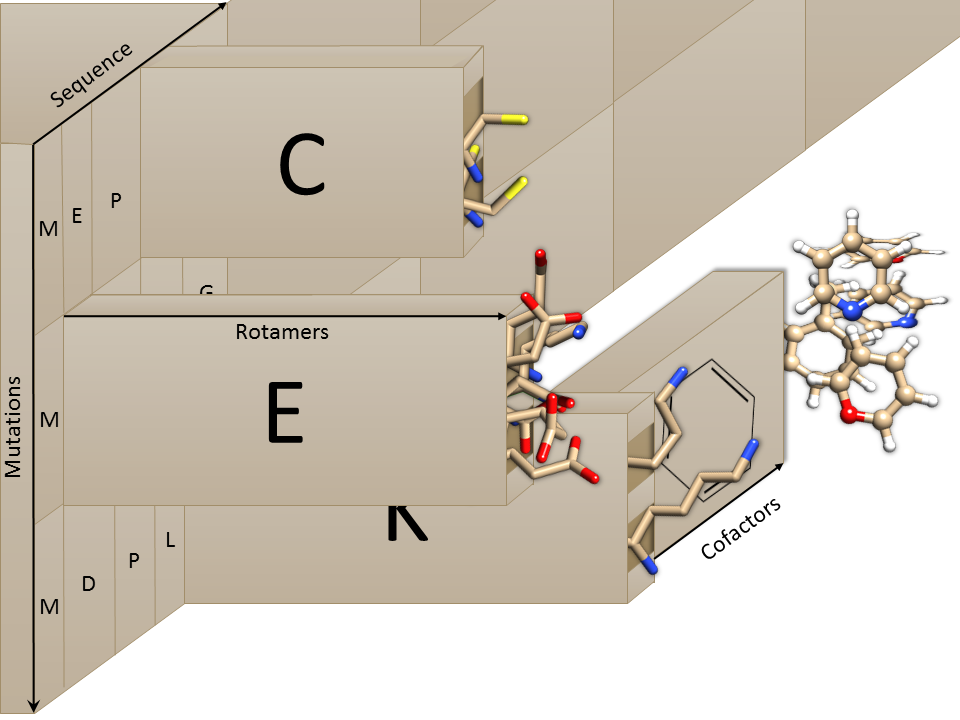
\includegraphics[width=\textwidth]{./figures/02/chemical_space.png}
	\caption[Chemobiological spaces]{
		In any study on protein-ligand interactions, considering sequence mutation of protein scaffolds, each with its possible sidechain orientations, already produces a combinatorial explosion. Taking different possible ligands into account adds one more dimension to the search space. (Reproduced from \textit{Rodríguez-Guerra, J., Alonso-Cotchico, L., Sciortino, G., Lledós, A., $\&$  Maréchal, J. D. (2018). Computational Studies of Artificial Metalloenzymes: From Methods and Models to Design and Optimization. Artificial Metalloenzymes and MetalloDNAzymes in Catalysis: From Design to Applications, 99-136}. $ \{ $ $ \} $ ).
	}
	\label{fig:chemicalspace}
\end{figure}

\subsubsection{Model/topology building}
% \addcontentsline{toc}{subsubsection}{Model/topology building}
Up to this point, it has been assumed that the molecular modeler had all the needed structures ready for analysis and simulation, but unfortunately that is not always the case.

In QM studies, when only small molecules are studied, manual building of the model can be contemplated as a possibility using a graphical interface $ \{ $ GaussView, Avogadro$ \} $ , but when the model grows, the possible orientation of rotatable bonds or the configuration of the subunits can be a daunting task to solve manually and even a stopping barrier in the research. Additionally, in some cases, the initial structure is only conceived as a 2D depiction with ChemDraw or similar software, which has to be transformed into a 3D model. This a fairly common process, and as such most software suites include a 2D->3D converter $ \{ $ $ \} $ . However, additional refinements are normally required afterwards.

In macromolecular studies where the conformational space is untreatable, experimental data is needed beforehand, like X-Ray Crystallography (XRC) or Nuclear Magnetic Resonance (NMR). These techniques provide density maps to which, with adequate refinement and post-processing using specialized software $ \{ $ CCP4, Phenix$ \} $ , 3D structures are fitted. After validating the quality of the resulting model with ERRAT or similar protocols $ \{ $ $ \} $ , these are then usually submitted to specialized databases like Protein Data Bank (PDB) $ \{ $ $ \} $ , from which the researchers can download the needed files for modelling the required system. Most of the time, files downloaded from PDB must be edited to remove experimental artefacts like duplicate positions of some atoms, protonate the residues at the desired pH by inferring the pKa of each one $ \{ $ Reduce, PropKa, \textit{addh}$ \ldots $ $ \} $ , or reproduce the biological assembly of the structure $ \{ $ SIENA, UCSF Chimera$ \} $ .

While the Protein Data Bank holds almost 140,000 structures readily available for everyone, not every protein is there. Sometimes, the structure is partially missing due to experimental limitations or even totally absent. In those cases, the model must be built from scratch. The folding problem is still unsolved and guessing the tertiary structure out of the sequence of amino acids is very challenging, but workarounds exist to work with available data. For example, if the protein that needs to be modelled has an already characterized homolog in the database, their sequence alignment can be used as a template to reconstruct a good structure. This technique is called homology modelling and its accuracy grows when multiple sequence alignment (MSA) are available. Since the final model is only an interpolation of closely related structures, some external validation is needed. In MODELLER, one of the most popular packages for homology modelling, several scoring functions to assess the quality are available. Additionally, a series of web services can be found to help in the task $ \{ $ ERRAT, QMEAN, APOLLO$ \ldots $  More on \href{https://www.click2drug.org/directory\_HomologyModeling.html}{https://www.click2drug.org/directory\_HomologyModeling.html}$ \} $ .\

\subsubsection{Cheminformatics}
% \addcontentsline{toc}{subsubsection}{Cheminformatics}
All previous techniques relied on 3D structural models of the involved compounds, but there are molecular modeling techniques that do not need to rely on that information to produce useful results.

Cheminformatics are mainly concerned with the creation and maintenance of small compound databases with support for indexation and similarity searches. The main exponent of cheminformatics approaches is probably Q\/SAR techniques.

Quantitative Structure-Activity Relationship (Q\/SAR) studies apply classification or regression statistical techniques to predict experimental observables from basic molecular descriptors. The\ ‘activity’ under study can comprise different variables: biological activity of a drug-like compound, boiling point, potential reactivity, toxicity$ \ldots $  All Q\/SAR methods are based on the structure-activity relationship (SAR) assumption: similar compounds will have similar activities. The main issue is how to measure that similarity: number of atoms, functional groups, connectivity$ \ldots $   As in all statistics, large datasets are needed to obtain valid results. The first step in Q\/SAR studies is to train the statistical model with a huge library of compounds. Once the model is trained, it can be used to predict the activity of a compound originally not present in the library.

Q\/SAR input data do not provide 3D-structural data (with the exception of the 3D-Q\/SAR variants), but 2D-topological information. These are normally supplied with special character strings called SMILES (Simplified Molecular Input Line Entry Specification) $ \{ $ $ \} $ , which can describe compounds unambiguously without resorting to explicit coordinates specification. SMILES strings work by enumerating the atoms involved in a molecule with their element symbol, except hydrogen, which is usually implicitly considered. Simple bonds are assumed between linearly adjacent elements. If a ramification occurs, it must be specified with parenthesis. Numeric tags are used to signal the starting and ending atoms of cyclic substructures (see fig. \ref{fig:smiles}). For example, butane would be represented as \texttt{CCCC}, while D-glucose would be \texttt{C(C1C(C(C(C(O1)O)O)O)O)O}.


\begin{figure}[H]
	\begin{center}
	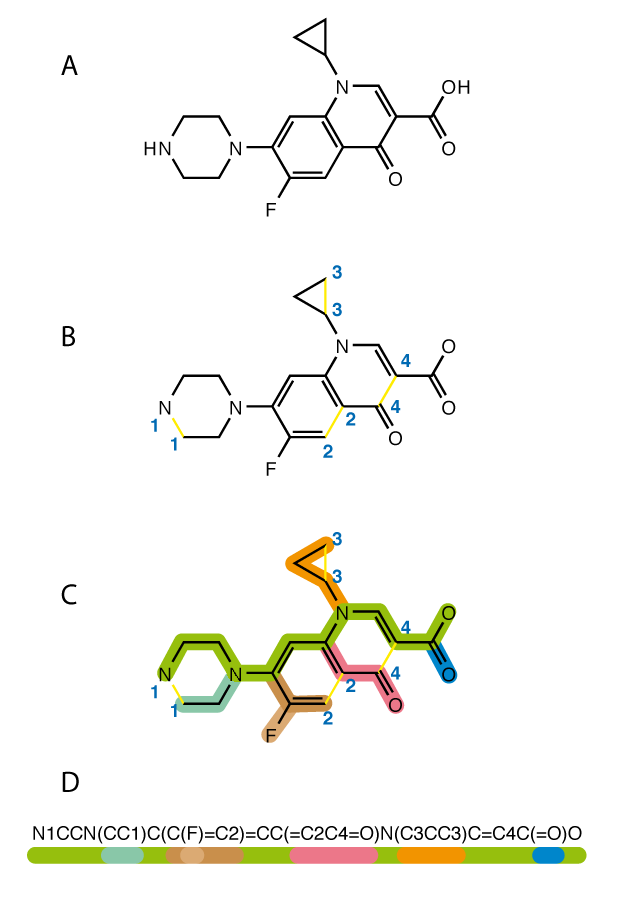
\includegraphics[height=0.9\textheight]{./figures/02/smiles.png}
	\end{center}
	\cprotect\caption[SMILES notation]{SMILES notation can depict a substituted aromatic ring as linear chains with branches. In this case, 3-cyanoanisole is being written as \texttt{COc(c1)cccc1C$\# $N}.}
	\label{fig:smiles}
\end{figure}


